\chapter[Transforming the Enriched Lambda Calculus][Transforming the Enriched Lambda Calculus]{Transforming the Enriched\\Lambda Calculus}
\vspace{3cm}

Having now defined the semantics of pattern-matching, we are in a position to
show how to transform all the constructs of the enriched lambda calculus into
the ordinary lambda calculus.

Section 6.1 shows how to transform pattern-matching lambda abstractions
into the ordinary lambda calculus, while Section 6.2 deals with let- and
letrec-expressions; Sections 6.3 and 6.4 deal with \ml{case}-expressions and the \fatbar{}
operator.

\section{Transforming Pattern-matching Lambda Abstractions}

In order to translate Miranda function definitions involving pattern-matching
into the enriched lambda calculus, we had to introduce pattern-matching
lambda abstractions as a new construct. In this section we will show how they
can be transformed into the ordinary lambda calculus. For each form of \ml{(\tlb{p}E)}
we will give an equivalent form that does not use pattern-matching lambda
abstractions.

In the case when the pattern \ml{p} is a variable there is nothing to do, because
no pattern-matching is involved. The remaining cases are when the pattern is
a constant, a product-constructor pattern or a sum-constructor pattern. These
are dealt with in the following three subsections.

\subsection{Constant Patterns}

This section shows how to transform a pattern-matching lambda abstraction
\ml{(\tlb{k}E)}, with a constant pattern \ml{k}, into the ordinary lambda calculus. First of
all, we recall the semantics of \ml{(\tlb{k}E)} from Section 4.3.2:

\begin{letalign}
\metafnbb{Eval}{\tlb{k}E} a = \metafnbb{Eval}{E} \qquad & \text{if} a $=$ \metafnbb{Eval}{k}\\
\metafnbb{Eval}{\tlb{k}E} a = FAIL &\text{if} a $\neq$ \metafnbb{Eval}{k}  \text{and} a $\neq \bot$  \\
\metafnbb{Eval}{\tlb{k}E} $\bot = \bot$
\end{letalign}
Operationally, \ml{(\tlb{k}E)} tests whether its argument is equal to \ml{k}; if so, it returns
\ml{E}, if not it returns \ml{FAIL}. This simple test can be carried out by the built-in \ml{IF}
function, using the following transformation:
\begin{mlcoded}
(\tlb{k}E) $\equiv$ (\tlb{v}   IF (= k v) E FAIL)
\end{mlcoded}
where \ml{v} is a new variable which does not occur free in \ml{E}. It should be clear
(and can be proved, using the semantics of  \ml{(\tlb{k}E)} and the semantics of \ml{IF} and
\ml{=}) that these two lambda abstractions have the same meaning, and hence are
equivalent. Notice the way in which we introduce a new \ml{\tl{v}} abstraction, so that
we can name the argument directly in its body.

As an example, consider the Miranda definition
\begin{mlcoded}
flip 0 = 1\\
flip 1 = 0
\end{mlcoded}
This will be translated to
\begin{mlcoded}
	\begin{tabular}{lll}
		flip = \tlb{x} &( &((\tlb{0} 1) x) \\
		& \fatbar{}  &((\tlb{1} 0) x) \\
		& \fatbar{} &ERROR)
	\end{tabular}
\end{mlcoded}
Now, transforming out the pattern-matching lambda abstractions gives
\begin{mlcoded}
	\begin{tabular}{lll}
		flip = \tlb{x} &( &((\tlb{v} IF (= 0 v) 1 FAIL) x) \\
		& \fatbar{}  &((\tlb{v} IF (= 1 v) 0 FAIL) x) \\
		& \fatbar{} &ERROR)
	\end{tabular}
\end{mlcoded}
It is now easy to verify that
\begin{mlcoded}
\begin{tabular}{llllll}
flip 0 & $\to$ & $\cdots$ & $\to$ & 1 \\
flip 1 & $\to$ & $\cdots$ & $\to$ & 0 \\
flip 2 & $\to$ & $\cdots$ & $\to$ & ERROR \\
\end{tabular}
\end{mlcoded}

\subsection{Product-constructor Patterns}

Next we consider the case of \ml{(\tlb{p}E)}, where \ml{p} is the product pattern
\ml{(t p$_1$ \ldots p$_r$)}, and \ml{t} is a product constructor of arity $r$. As before, we recall its
semantics (Section 4.3.4):
\begin{letalign}
	\metafnbb{Eval}{\tlb{(t p$_1$ $\ldots$ p$_r$)}E} a = \metafnbb{Eval}{ \tl{p$_1$} $\ldots$ \tlb{p$_r$}E } & (SEL-t-1 a)\\
	& $\cdots$\\
	& (SEL-t-r a)
\end{letalign}

To implement this semantics, we invent a new function
\ml{UNPACK-PRODUCT-t} for each product constructor \ml{t}, and use it in this
transformation:
\begin{mlcoded}
(\tlb{(t p$_1$ $\ldots$ p$_r$)}E) $\equiv$ UNPACK-PRODUCT-t (\tl{p$_1$}$\ldots$\tlb{p$_r$}E)
\end{mlcoded}
The idea is that \ml{UNPACK-PRODUCT-t} takes two arguments, a function and a
structured object, and applies the function to the lazily selected components
of the object. It is defined by the following semantic equation:
\begin{mlcoded}
UNPACK-PRODUCT-t f a $=$ f (SEL-t-1 a) $\cdots$ (SEL-t-r a)
\end{mlcoded}
It can easily be shown that the transformation is valid, by comparing the
semantics of the expression before and after the transformation.

The right-hand side of the transformation still has pattern-matching lambda
abstractions in it, but they are smaller than the one we began with, and
repeated use of the rules for transforming pattern-matching lambda
abstractions will eliminate them.

As an example, consider the function \ml{addPair}, which adds together the
elements of a pair:
\begin{mlcoded}
	addPair = \tlb{PAIR x y} + x y
\end{mlcoded}
This will be transformed to
\begin{mlcoded}
	addPair = UNPACK-PRODUCT-PAIR (\tlb{x}\tlb{y}+ x y)
\end{mlcoded}
We can check that it gives the right results by reducing \ml{(addPair (PAIR 3 4))}:
\begin{mlcoded}
	addPair (PAIR 3 4)\\
	\phantom{--}= UNPACK-PRODUCT-PAIR (\tlb{x}\tlb{y}+ x y) (PAIR 3 4) \\
	$\rightarrow$ (\tlb{x}\tlb{y}+ x y) (SEL-PAIR-1 (PAIR 3 4)) (SEL-PAIR-2 (PAIR 3 4)) \\
	$\rightarrow$ (\tlb{y}+ (SEL-PAIR-1 (PAIR 3 4)) y) (SEL-PAIR-2 (PAIR 3 4)) \\
	$\rightarrow$ + (SEL-PAIR-1 (PAIR 3 4)) (SEL-PAIR-2 (PAIR 3 4)) \\
	$\rightarrow$ + 3 (SEL-PAIR-2 (PAIR 3 4)) \\
	$\rightarrow$ + 3 4 \\
	$\rightarrow$ 7
\end{mlcoded}

\subsection{6.1.3 Sum-constructor Patterns}

Finally, consider the case of \ml{(\tlb{p}E)}, where \ml{p} is a sum pattern \ml{(s p$_1$ $\cdots$ p$_r$)}, and
\ml{s} is a sum constructor of arity \ml{r}. The semantics of such lambda abstractions
was derived in Section 4.3.3:
\begin{letalign}
	\metafnbb{Eval}{\tlb{(s p$_1$\,\ldots\,p$_r$)}E} (s a$_1$\,\ldots\,a$_r$)
	&= \metafnbb{Eval}{\tl{p$_1$}\ldots\tlb{p$_r$}E} a$_1$\,\ldots\,a$_r$ \\
	\metafnbb{Eval}{\tlb{(s p$_1$\,\ldots\,p$_r$)}E} (s$'$ a$_1$\,\ldots\,a$_{r'}$)
	&= FAIL \qquad {\normalfont if} s$\,\neq\,$s$'$ \\
	\metafnbb{Eval}{\tlb{(s p$_1$\,\ldots\,p$_r$)}E} $\bot$
	&= $\bot$ \\
\end{letalign}


We can make a very similar transformation to the product-constructor case,
leaving all the hard work to a new function \ml{UNPACK-SUM-s}:
\begin{mlcoded}
	(\tlb{(s p$_1$\,\ldots\,p$_r$)}E) $=$ UNPACK-SUM-s (\tl{p$_1$}\,\ldots\,\tlb{p$_r$}E)
\end{mlcoded}

The function \ml{UNPACK-SUM-s} takes two arguments, a function (in this case
\ml{(\tl{p$_1$} \ldots \tlb{p$_r$}. E)}), and a structured object. It checks whether the object is built
with constructor \ml{s}: if not, \ml{FAIL} is returned; if so, \ml{UNPACK-SUM-s} takes the
object apart and applies the function (its first argument) to its components.
\ml{UNPACK-SUM-s} is specified by the following semantic equations:
\begin{letalign}
	UNPACK-SUM-s f (s a$_1$\,\ldots\,a$_r$) &= f\,a$_1$\,\ldots\,a$_r$ \\
	UNPACK-SUM-s f (s$'$ a$_1$\,\ldots\,a$_{r'}$) &= FAIL \qquad {\normalfont if} s\,$\neq$\,s$'$\\
	UNPACK-SUM-s f $\bot$ &= $\bot$
\end{letalign}

As an example, recall the Miranda definition of \ml{reflect}:
\begin{letalign}
	reflect (LEAF n) &= LEAF n\\
	reflect (BRANCH t$_1$ t$_2$) &= BRANCH (reflect t$_2$) (reflect t$_1$)
\end{letalign}
This is translated to:
\begin{mlalign}
	reflect = \tlb{t}&( ((\tlb{(LEAF\ n)}LEAF\ n) t)\\
	&\fatbar{} ((\tlb{(BRANCH t$_1$\ t$_2$)}BRANCH (reflect\ t$_2$) (reflect\ t$_1$)) t)\\
	&\fatbar{}  ERROR)
\end{mlalign}
Now, applying the transformation gives:
\begin{mlalign}
	reflect\\
	= \tl{t}. &( (UNPACK-SUM-LEAF (\tl{n}. LEAF\ n) t)\\
	&\fatbar{}  (UNPACK-SUM-BRANCH (\tlb{t$_1$}\tlb{t$_2$}BRANCH (reflect\ t$_2$) (reflect\ t$_1$)) t)\\
	&\fatbar{}  ERROR)
\end{mlalign}

\subsection{Reducing the Number of Built-in Functions}

The trouble with the transformations of the previous section is that they
introduce several functions associated with each constructor. In this section,
we discuss the implementation of these functions.

A structured object will be represented by the implementation as an
aggregate, consisting of the component fields together with a \textit{structure tag},
which distinguishes objects built by different constructors from each other
(see Section \ml{10.3.1}). It is this tag which can be used by \ml{UNPACK-SUM-s} to
identify the constructor used.

In a type-checked system, it is only necessary to distinguish objects from
other objects of the same type, so the structure tag can be a small integer in the
range \ml{1} \ldots \ml{n} (where \ml{n} is the number of constructors in the type). This means
that, instead of requiring an \ml{UNPACK-SUM-s} function for each constructor \ml{s},
it is only necessary to have a single family of functions \ml{UNPACK-SUM-d-r$_s$},
where \ml{d} is the integer structure tag which is recognized by \ml{UNPACK-SUM-d-r$_s$},
and \ml{r$_s$} is the arity of \ml{s}. In a similar way, the sum constructor functions can be
replaced with a family of functions \ml{PACK-SUM-d-r$_s$}, which take \ml{r$_s$} arguments
and construct an aggregate with \ml{r$_s$} fields and structure tag \ml{d}.

We can perform an analogous set of replacements for the functions
associated with product types. \ml{UNPACK-PRODUCT-t} can be replaced with
\ml{UNPACK-PRODUCT-r$_t$}, where \ml{r} is the arity of \ml{t} (there is no need for a structure
tag here, since \ml{UNPACK-PRODUCT} does not examine it). Similarly, the
product-constructor functions can be replaced with \ml{PACK-PRODUCT-r$_t$}, and
the selector functions \ml{SEL-t-i} can be replaced with \ml{SEL-r$_{t}$-i}. It is sensible to
keep \ml{PACK-SUM} and \ml{PACK-PRODUCT} distinct because, having no structure
tag, objects of product type may have a different representation from objects
of sum type.

To summarize:
\vspace{0.5\baselineskip}

{\setlength{\tabcolsep}{1pt}
\begin{tabular}{rl}
	\ml{s} (a sum-constructor function) &is replaced by \ml{PACK-SUM-d-r$_s$}\\
	\ml{UNPACK-SUM-s} &is replaced by \ml{UNPACK-SUM-d-r$_s$}\\
	\ml{t} (a product-constructor function) &is replaced by \ml{PACK-PRODUCT-r$_t$}\\
	\ml{UNPACK-PRODUCT-t} &is replaced by \ml{UNPACK-PRODUCT-r$_t$}\\
	\ml{SEL-t-i} &is replaced by \ml{SEL-r$_{t}$-i}
\end{tabular}

\begin{tabular}{rl}
where \ml{r$_s$} &$=$ arity of \ml{s},\\
\ml{d} &$=$ structure tag of \ml{s},\\
\ml{r$_t$} &$=$ arity of \ml{t}.\\
\end{tabular}
}
\vspace{0.5\baselineskip}

For example, assuming that we implement lists with structure tag $1$ for \ml{NIL}
and $2$ for \ml{CONS}, then the following replacements would take place:
\vspace{0.5\baselineskip}

{\setlength{\tabcolsep}{1pt}
	\begin{tabular}{rl}
	\ml{NIL} &is replaced by \ml{PACK-SUM-1-0}\\
	\ml{CONS} &is replaced by \ml{PACK-SUM-2-2}\\
	\ml{UNPACK-SUM-NIL} &is replaced by \ml{UNPACK-SUM-1-0}\\
	\ml{UNPACK-SUM-CONS} &is replaced by \ml{UNPACK-SUM-2-2}
\end{tabular}
}
\vspace{0.5\baselineskip}

Likewise, if the type \ml{tree} is declared as before:
\begin{mlcoded}
	tree ::= LEAF num | BRANCH tree tree
\end{mlcoded}
and \ml{LEAF} and \ml{BRANCH} are assigned structure tags 1 and 2 respectively, the
following replacements would take place:
\vspace{0.5\baselineskip}

{\setlength{\tabcolsep}{1pt}
\begin{tabular}{rl}
	\ml{LEAF} &is replaced by \ml{PACK-SUM-1-1}\\
	\ml{BRANCH} &is replaced by \ml{PACK-SUM-2-2}\\
	\ml{UNPACK-SUM-LEAF} &is replaced by \ml{UNPACK-SUM-1-1}\\
	\ml{UNPACK-SUM-BRANCH} &is replaced by \ml{UNPACK-SUM-2-2}
\end{tabular}
}\vspace{0.5\baselineskip}

Finally, if the type \ml{pair} is declared as before:
\begin{mlcoded}
	pair $*$ $**$ ::= PAIR $*$ $**$
\end{mlcoded}
the following replacements would take place:
\vspace{0.5\baselineskip}

{\setlength{\tabcolsep}{1pt}
	\begin{tabular}{rl}
	\ml{PAIR} &is replaced by \ml{PACK-PRODUCT-2}\\
	\ml{UNPACK-PRODUCT-PAIR} &is replaced by \ml{UNPACK-PRODUCT-2}\\
	\ml{SEL-PAIR-1} &is replaced by \ml{SEL-2-1}\\
	\ml{SEL-PAIR-2} &is replaced by \ml{SEL-2-2}
\end{tabular}
\vspace{0.5\baselineskip}

Since functions with different types may be replaced by the same function
(for example, \ml{CONS} and \ml{BRANCH} are both replaced by \ml{PACK-SUM-2-2}), these
replacements should not be performed until after type-checking. For the
same reason, none of these replacements is possible for a system that
performs run-time type-checking (see Section 10.5).

\subsection{Summary}
Figure 6.1 summarizes the transformations developed in this section, and
Figure 6.2 gives the semantics for the two new families of functions we
introduced in order to perform the transformations.


\boxedfigure{
	\begin{mlcoded}
	\begin{tabular}{lll}
			(\tlb{k}E)	& $\equiv$  (\tlb{v} IF (= k v) E FAIL) \\
			&  \phantom{ $\equiv$  } {\normalfont where} v {\normalfont is a new variable that does not } \\
			&	\phantom{ $\equiv$  } \qquad{\normalfont occur free in} E\\
			(\tlb{(t p$_1$ \ldots p$_{r_t}$)E}) & $\equiv$ (UNPACK-PRODUCT-t (\tlb{p$_1$ \ldots p$_{r_t}$ E})) \\
			(\tlb{(s p$_1$ \ldots p$_{r_s}$) E}) & $\equiv$ (UNPACK-SUM-s (\tlb{p$_1$ \ldots p$_{r_s}$ E}))
	\end{tabular}
	\end{mlcoded}

		\begin{tabular}{lll}
			where	& \ml{k}  & is a constant \\
			& \ml{t} & is a product constructor of arity \ml{r$_t$}\\
			& \ml{s} & is a sum constructor of arity \ml{r$_s$}
		\end{tabular}
}{Transforming out pattern-matching lambda abstractions}


\boxedfigure{
	\begin{mlcoded}
		UNPACK-PRODUCT-t f a = f (SEL-t-1 a) \ldots (SEL-t-r$_t$ a) \\

		\begin{tabular}{lll}
			UNPACK-SUM-s f (s a$_1$ \ldots a$_{r_s}$) &= f a$_1$ \ldots a$_{r_s}$ \\
			UNPACK-SUM-s f (s' a$_1$ \ldots a$_{r_{s'}}$) &= FAIL  \qquad {\normalfont if} s\,$\neq$\,s$'$\\
			UNPACK-SUM-s f $\bot$ &=$\bot$
		\end{tabular}
	\end{mlcoded}

	\begin{tabular}{lll}
		where & \ml{t} & is a product constructor of arity \ml{r$_t$}\\
		& \ml{s} & is a sum constructor of arity \ml{r$_s$}
	\end{tabular}
}{Semantics of \ml{UNPACK-PRODUCT} and \ml{UNPACK-SUM}}


\section{Transforming \ml{let} and \ml{letrec}}

In Section 4.2.9 we introduced a new complication to \ml{let}(\ml{rec})-expressions, by
allowing the left-hand side of definitions to be an arbitrary pattern rather than
a simple variable. In this section we show how to transform these generalized
\ml{let}s and \ml{letrec}s into successively simpler forms, arriving eventually at the
ordinary lambda calculus.

Rather than defining the semantics of \ml{let} and \ml{letrec} directly, as we did for
pattern-matching lambda abstractions, we will regard the transformations
described in this section as a definition of their semantics. To define their
meaning in a more direct way would require more mathematical machinery
than we have available in this book.

We begin by sketching a new problem which is introduced by allowing
arbitrary patterns on the left-hand side of definitions. This leads us to define a
class of patterns, the \textit{irrefutable} patterns, which do not suffer from the
problem. Then, before embarking on the transformations themselves, we
give a 'map' to explain their structure.

\subsection{Conformality Checking and Irrefutable Patterns}

Allowing arbitrary patterns on the left-hand side of a definition introduces a
new and somewhat subtle complication. Consider the expression
\begin{mlcoded}
	let (CONS x xs) = B in E
\end{mlcoded}
Here, the pattern \ml{(CONS x xs)} appears on the left-hand side of the definition.
This raises the nasty possibility that B might evaluate to \ml{NIL} instead of
\ml{(CONS B$_1$ B$_2$)}, in which case the pattern would not match, and some sort of
error should, presumably, be reported. This requires that a \textit{conformality
check} be made, to ensure that B conforms with the specified pattern.
Conformality checking will carry some implementation cost, so we would
like to avoid it whenever possible. It can be avoided in precisely those cases
when the pattern match cannot fail; for example, simple product patterns.
However, there are some nested patterns which cannot fail also, which
motivates the following definition:


\simpletitledbox{DEFINITION}{
A pattern \ml{p} is \textit{irrefutable} if it is
\begin{numbered}
	\item either a variable \ml{v}
	\item or a product pattern of form \ml{(t p$_1$ \ldots p$_{r_t}$)} where \ml{p$_1$}, \ldots, \ml{p$_{r_t}$} are irrefutable patterns.
\end{numbered}
Otherwise the pattern is \textit{refutable}.
}

\noindent In other words, the irrefutable patterns consist of arbitrarily nested product
constructors with variables at the leaves. These patterns cannot fail to match
in a type-checked implementation. Variables and simple product patterns are
just two examples of irrefutable patterns.

However, even a single constant or sum constructor (even if nested inside a
product pattern) makes the pattern refutable, since there is a possibility that it
may not match. We need to perform conformality checking for refutable
definitions only.

\subsection{Overview of let and letrec Transformations}
We are now ready to describe the various transformations to simplify \ml{let}(\ml{rec})-
expressions. While few are complicated, they are quite numerous, so we
begin by offering a `map' to aid in navigation through the rest of the section.

For a start, we establish the following terminology:
\begin{numbered}
	\item The left-hand side of each definition of a simple \ml{let(rec)}-expression must
	be a variable.
	\item The left-hand side of each definition of an irrefutable \ml{let(rec)}-expression
	must be an irrefutable pattern.
	\item The left-hand side of each definition of a general \ml{let(rec)}-expression may
	be any arbitrary pattern.
\end{numbered}
With the aid of this terminology, Figure 6.3 depicts the transformations which
will be described below, giving the appropriate section number in brackets.

For the reasons discussed in Section 3.2.4, there are two possible forms into
which we may wish to transform the program, which differ only in their
treatment of \ml{let} and \ml{letrec}:
\begin{numbered}
	\item We may transform the program into the ordinary lambda calculus; this
	gives the simplest resulting program. In this case, general \ml{let}s are trans-
	formed into the ordinary calculus via irrefutable \ml{let}s and simple \ml{let}s.
	General \ml{letrec}s, on the other hand, are first transformed into irrefutable
	\ml{let}s via irrefutable \ml{letrec}s, and then use the \ml{let} transformations.
	\item We may transform the program into the ordinary lambda calculus
	augmented with simple \ml{let(rec)}-expressions; the resulting program is
	slightly more complicated, but can be implemented more efficiently
	(Section 3.2.4). In this case, general \ml{let}s are transformed only into simple
	\ml{let}s, and general \ml{letrec}s are transformed into simple \ml{letrec}s, via irrefutable
	\ml{letrec}s.
\end{numbered}

\begin{figure}[H]
	\centering

	\fbox{%
		\begin{minipage}{0.9\textwidth}
			\small
			\setlength{\parindent}{10pt}
			\setlength{\parskip}{0mm plus 0mm minus 0mm}

			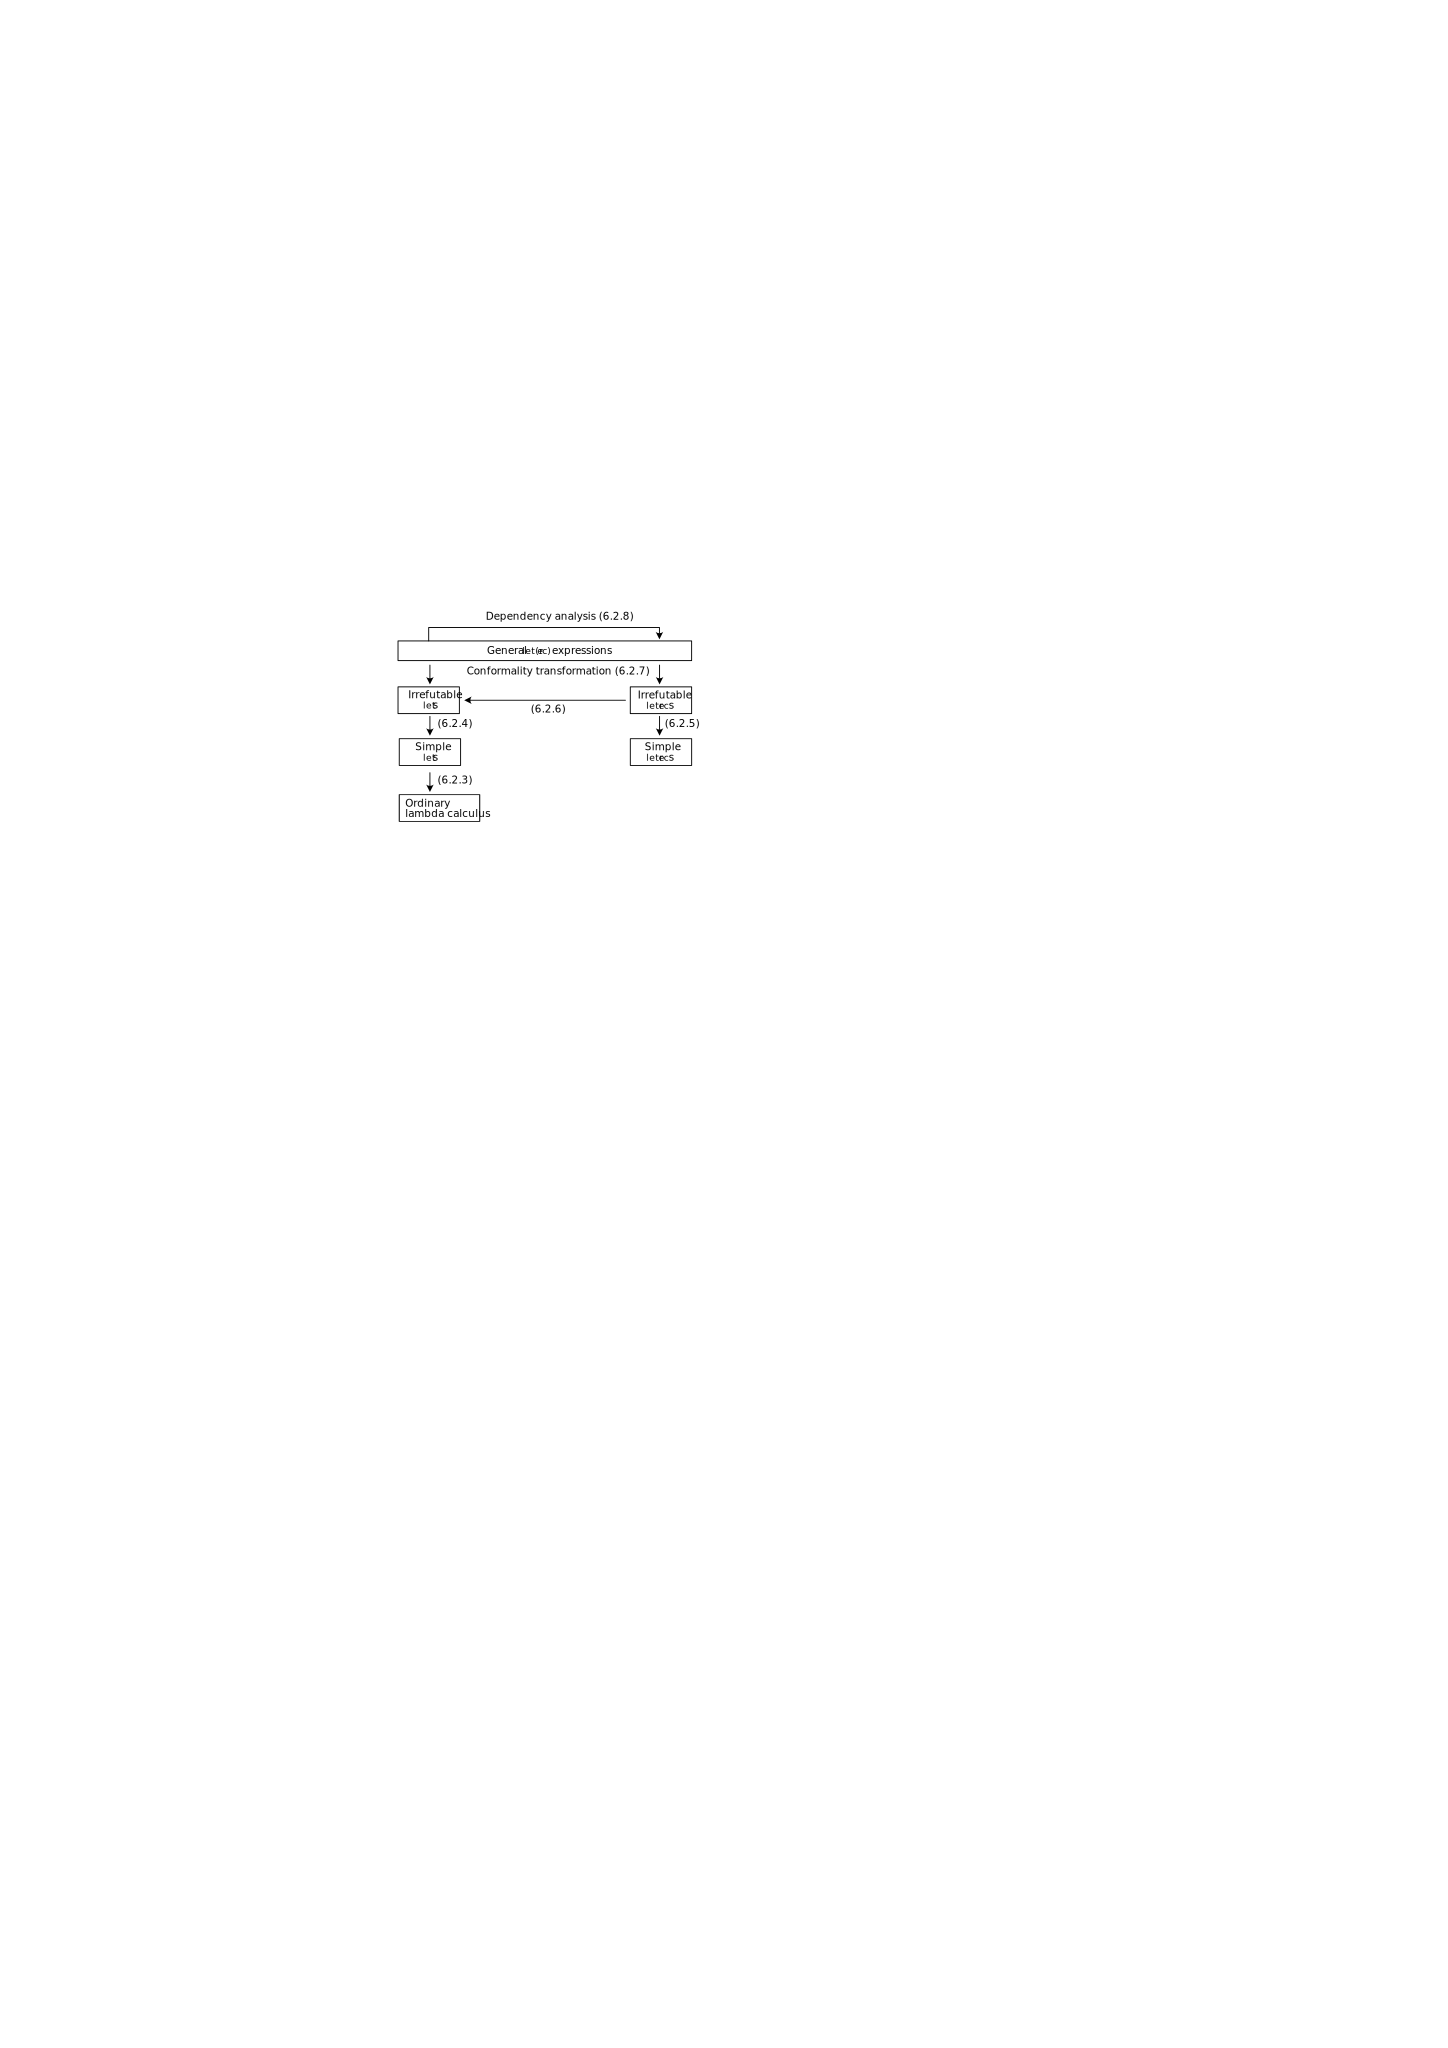
\includegraphics[width=0.96\textwidth]{chapters/Fig6_3}
			%                    \includesvg{chapters/Fig3_4}
			%                    \input{chapters/Fig3_4.tex}

		\end{minipage}%

	}%

	\caption{\textsf Map of \ml{let(rec)} transformations}
\end{figure}

\noindent Both possibilities are catered for by the transformations shown in Figure 6.3.

In what follows, when considering \ml{let}-expressions we assume that they
contain only one definition. This gives no loss of generality, since a \ml{let}-expression with multiple definitions is trivially equivalent to a nested set of
single-definition \ml{let}-expressions.

The following sections deal with the transformations depicted in Figure 6.3.

\subsection{Transforming Simple \ml{let}s into the Ordinary Lambda Calculus}

Once we have arrived at an expression in which all \ml{let}-expressions are simple,
it is easy to remove them altogether, using the transformation given in Section
3.2.1:

\plainbox{
\begin{mlcoded}
	let v = B in E $\equiv$ (\tlb{v}E) B
\end{mlcoded}
}
\noindent For example,
\begin{mlcoded}
	let x = 4 in (+ x 6) $\equiv$ (\tlb{x}+ x 6) 4
\end{mlcoded}

\subsection{Transforming Irrefutable \ml{let}s into Simple \ml{let}s}

Consider the case of an irrefutable \ml{let}-expression, of the form
\begin{mlcoded}
	let p = B in E
\end{mlcoded}
where \ml{p} is irrefutable. Since the pattern on the left-hand side of the definition
is irrefutable, it must either be a variable or a product pattern. In the former
case, there is nothing to do, since the \ml{let}-expression is already simple. In the
latter case, the \ml{let}-expression takes the form
\begin{mlcoded}
	let (t p$_1$ \ldots p$_r$) = B in E
\end{mlcoded}
where the \ml{p$_i$} are irrefutable patterns, and \ml{B} and \ml{E} are expressions. We can now
make the following transformation:

\plainbox{
\begin{mlcoded}
	\begin{tabular}{llll}
	let (t p$_1$ \ldots p$_r$) = B in E $\equiv$ \ &let &v =&\ B \\
		&in &(let &p$_1$ = SEL-t-1 v \\
		& & &\ldots \\
		& & &p$_r$ = SEL-t-r v \\
		& & \;\;in &E)
	\end{tabular}
\end{mlcoded}
where \ml{v} is a new variable that does not occur free in \ml{E}.
}

The \ml{p$_i$} are bound to selector functions applied to \ml{v}, which is in turn bound to
\ml{B}. Repeated application of this transformation will eliminate all non-simple
irrefutable \ml{let}-expressions.

To take an example, the expression
\begin{mlcoded}
	let (PAIR x y) = B in E
\end{mlcoded}
would be transformed to
\begin{mlcoded}
	\begin{tabular}{lll}
	let v = B in (&let &x = SEL-PAIR-1 v \\
		& &y = SEL-PAIR-2 v\\
		&in &E)
	\end{tabular}
\end{mlcoded}

Notice that if neither \ml{x} nor \ml{y} is evaluated in \ml{E}, then \ml{B} will not be evaluated
either, so the transformation implements lazy product-matching. Lazy
product-matching is just as much of an advantage here as it was in function
definitions. For example, we could recode the function \ml{firsts} from Section
4.3.5 in the following way:
\begin{mlcoded}
	\begin{tabular}{lll}
	firsts [\,] &= &(0, 0)\\
	firsts (x:xs) &= &(x, ev), \qquad odd x\\
	&= &(od, x), \qquad even x\\
	& &where\\
	& &(od, ev) = firsts xs
	\end{tabular}
\end{mlcoded}
We would expect this definition to behave just like that of Chapter 4, so that if
lazy product-matching is used for function definitions then it should also be
used for \ml{let}(\ml{rec})-expressions.

(Note: an alternative transformation would have been possible in this
section, namely:
\begin{mlcoded}
	let p = B in E = (\tlb{p}E) B
\end{mlcoded}
where \ml{p} is an irrefutable pattern. From a semantic point of view, this is
entirely equivalent to the transformation used above. However, for the
efficiency reasons outlined in Section 3.2.4, we prefer to stay in the world of
\ml{let}-expressions as long as possible; hence our choice.)

\subsection{Transforming Irrefutable \ml{letrec}s into Simple \ml{letrec}s}

The transformation from a letrec involving only irrefutable definitions into a
simple \ml{letrec} is very similar to that for \ml{let}-expressions:

\plainbox{
\begin{mlcoded}
	\begin{tabular}{llll}
	letrec &(t p$_1$ \ldots p$_r$) = B $\equiv$ &letrec &v = B \\
	&<other definitions> & & p$_1$ = SEL-t-1 v \\
	in E & & & $\cdots$\\
	&  & &	p$_r$ = SEL-t-r v \\
	& &	& <other definitions>\\
	& & in E &
	\end{tabular}
\end{mlcoded}
\quad where \ml{v} is a new variable that does not occur free in \ml{E} or \ml{B}.
}


All the transformed definitions must be in a single \ml{letrec}, to ensure that
variables in the patterns \ml{p$_i$} are in scope in \ml{B}. The `\ml{<other definitions>}' simply
takes into account the fact that the \ml{letrec} may contain multiple definitions, and
this transformation should be applied to each of them separately.

Repeated application of the transformation will simplify the \ml{p$_i$} successively,
until the \ml{letrec} is simple.

\subsection{Transforming Irrefutable letrecs into Irrefutable lets}

In showing how to eliminate \ml{letrec}-expressions altogether, we could take as
our starting-point the simple \ml{letrec}-expressions produced by the transformation
described in the preceding section. However, it is slightly more efficient
to start from an earlier stage, the irrefutable \ml{letrec}-expressions.

First of all, we recall from Section~3.2.2 how to transform a simple \ml{letrec}
containing only a single definition:
\begin{mlcoded}
(letrec v = B in E)\equivalent (let v = Y (\tlb{v}B) in E)
\end{mlcoded}
We simply use the built-in function \ml{Y}, which was introduced in Section~2.4, to
make the definition non-recursive. Now that the definition is non-recursive,
we can use \ml{let} instead of \ml{letrec}, and the job is done.

When there is more than one definition, we apply the following sequence of
two transformations. First of all, we apply the transformation

\plainbox{
	\begin{mlcoded}
		\begin{tabular}{lll}
			letrec &p$_1$ = B$_1$ &\equivalent letrec (t p$_1$ \ldots{} p$_n$) = (t B$_1$ \ldots{} B$_n$) in E \\
			&\ldots &\\
			&P$_n$ = B$_n$ &\\
			in &E&
		\end{tabular}
	\end{mlcoded}
	\quad where \ml{t} is a product constructor of arity $n$.
}
\noindent In other words, we simply package up the right-hand sides into a tuple and
match it against a product pattern on the left-hand side. Furthermore, since
the \ml{p$_i$} are irrefutable, the pattern \ml{(t p$_1$ \ldots{} p$_n$)} is also irrefutable.

Now the \ml{letrec} contains only a single definition with an irrefutable pattern
on its left-hand side, and we can proceed by analogy with the simple case
described above, using \ml{Y}. This analogy yields the following transformation:

\plainbox{
\begin{mlcoded}
letrec p = B in E \equivalent let p = Y (\tlb{p}B) in E
\end{mlcoded}
\quad where \ml{p} is an irrefutable pattern.
}
\ml{Y} is used exactly as before, to make the definition non-recursive. The new
feature is the use of a pattern-matching lambda abstraction, where we used
only a simple lambda abstraction before. The result is a \ml{let}-expression with an
irrefutable pattern on its left-hand side, which is therefore amenable to the
transformations of Section~6.2.4.

To see this transformation in action, consider the following \ml{letrec}-expression:
\begin{mlcoded}
	\begin{tabular}{ll}
		letrec &x = CONS 1 y\\
		&y = CONS 2 x\\
		in x&
	\end{tabular}
\end{mlcoded}
It defines the infinite list \ml{[1,2,1,2, \ldots]}. Applying the first transformation, we
package up the definitions into one:
\begin{mlcoded}
		letrec (PAIR x y) = PAIR (CONS 1 y) (CONS 2 x) in x
\end{mlcoded}
Now, applying the second transformation gives:
\begin{mlcoded}
		let (PAIR x y) = Y (\tlb{(PAIR x y)}PAIR (CONS 1 y) (CONS 2 x)) in x
\end{mlcoded}
It is vital that the pattern-matching lambda abstraction should use lazy
product-matching. If it were to use strict product-matching instead, the
expression would yield \ml{1} rather than \ml{[1, 2, 1, 2, \ldots]}. In fact, mutual recursion
cannot be implemented using \ml{Y} without some form of lazy product-matching.

Using the transformations for \ml{let}-expressions and pattern-matching lambda
abstractions, we could complete the transformation of the current example as
follows:
\begin{mlcoded}
(\tlb{v}(\tlb{x}\tlb{y}x) (SEL-PAIR-1 v) (SEL-PAIR-2 v)) \\
(Y (UNPACK-PRODUCT-PAIR (\tlb{x}\tlb{y}PAIR (CONS 1 y) (CONS 2 x))))
\end{mlcoded}
This expression is not a pretty sight, but it gives the correct answer (that is, the
infinite list \ml{[1, 2, 1, 2, 1, 2, \ldots]}).

It should be clear from this example that implementing \ml{letrec} using tuples
carries a run-time cost, both to build the tuple and to take it apart. This is one
of the reasons why more sophisticated implementations implement simple
\ml{let}(\ml{rec})s directly (see Section~3.2.4 and Chapter~14).

\subsection{Transforming General let(rec)s into Irrefutable let(rec)s}

In Miranda, arbitrary patterns may appear on the left-hand side of a
definition. For example, consider the following Miranda definition of the
function \ml{head}, which extracts the first element of a list:
\begin{mlcoded}
	\begin{tabular}{ll}
		head xs = &y\\
		&where (y:ys) = xs
	\end{tabular}
\end{mlcoded}
The pattern \ml{(y:ys)} appears on the left-hand side of the definition in the
\ml{where}-clause. But this raises an awkward question: what would happen if the
pattern \ml{(y:ys)} did not match the result of evaluating \ml{xs}? In particular, what
would happen if we evaluated \ml{(head [\;]\,)}?

It is clearly unacceptable for the system to proceed in ignorance that
anything is wrong, so it is necessary to check that \ml{xs} matches the pattern,
rather than assume that it always will. This is called the \textit{conformality check},
since it checks that \ml{xs} conforms to the pattern.

Notice that the possibility of a mismatch only arises in the case of refutable
patterns, involving sum-constructor patterns or constants. The irrefutable
patterns, involving variables and product-constructor patterns only, cannot
fail to match (in a type-checked implementation).

The translation into the enriched lambda calculus does not affect the
problem of conformality checking. For example, the definition of \ml{head}
translates to:
\begin{mlcoded}
head = \tlb{xs}(letrec (CONS y ys) = xs in y)
\end{mlcoded}
The pattern \ml{(CONS y ys)} is refutable, and may fail to match. The problem
applies equally to \ml{let}s and \ml{letrec}s.

Having decided that conformality checking is essential, the next question
is: when is the conformality check performed? There are two possible
answers:
\begin{numbered}
	\item When the evaluation of the entire \ml{let(rec)}-expression begins.
	\item On the first occasion when either \ml{y} or \ml{ys} is used.
\end{numbered}
To illustrate the consequences of this choice, consider the (rather
contrived) expression
\begin{mlcoded}
let (CONS y ys) = NIL in 6
\end{mlcoded}
The first answer specifies that the evaluation of this expression should cause
an error, while the second specifies that it should return \ml{6}.

In keeping with its lazy approach, the semantics of Miranda specifies the
second of the two answers, and so this property should be inherited by
\ml{let(rec)}-expressions. How is this to be achieved? The simplest way seems to be
to transform the expression
\begin{mlcoded}
let (CONS y ys) = B in E
\end{mlcoded}
into
\begin{mlcoded}
		let (PAIR y ys) = (((\tlb{(CONS y ys)}PAIR y ys) B) \fatbar{} ERROR) in E
\end{mlcoded}
and rely on the transformation of Section~6.2.5 to cope with the simple product
pattern \ml{(PAIR y ys)}. The expression on the right-hand side will evaluate \ml{B}, check
that it is an object constructed with \ml{CONS}, take it apart, and construct a pair
containing its two components. These components are then bound to \ml{y} and \ml{ys} using
a simple product pattern on the left-hand side.

If it is not an object constructed with \ml{CONS}, then the application of the
pattern-matching lambda abstraction to \ml{B} will return \ml{FAIL}, and \ml{I} will return its
second argument, namely \ml{ERROR}.

There are two points to notice about this transformation:
\begin{numbered}
	\item No conformality check will be made if neither \ml{y} nor \ml{ys} is used in \ml{E},
	because the lazy product-matching ensures that the right-hand side of the
	definition is not evaluated unless at least one of the components of the
	tuple is used.
	\item The conformality check is made at most once. The evaluation of \ml{y} or \ml{ys}
	will cause the evaluation of the right-hand side of the definition, at which
	point the conformality check will be made, and the tuple built. Now,
	further use of \ml{y} or \ml{ys} will simply access the components of this tuple.
\end{numbered}

It seems hard to improve on these two properties, so we now generalize the
method to handle any \ml{let(rec)}-expression. Given a definition of the form
\ml{p = B}
where \ml{p} is a refutable pattern, we use the following transformation:
\begin{mlcoded}
p = B \equivalent (t v$_1$ \ldots v$_n$) = ((\tlb{p}(t v$_1$ \ldots v$_n$)) B) \fatbar{} ERROR
\end{mlcoded}
where \ml{t} is a product constructor of arity \ml{n}. The resulting definition now has an
irrefutable pattern on the left-hand side. We call this the \textit{conformality
transformation}, and it applies separately to any definition in a \ml{let} or \ml{letrec}
which has a refutable pattern on the left-hand side.

The variables \ml{v$_1$ \ldots v$_n$} are simply the variables that appear anywhere in the
pattern \ml{p}. This suggests a new definition.

\definitionbox{For any pattern \ml{p}, the set of variables of \ml{p}, abbreviated \ml{Var(p)}, is defined
	thus:
}{%
	{%
	\leftskip=1cm

\noindent if \ml{p} is a variable \ml{v}, then \ml{Var(p) = \{v\}}\\
if \ml{p} is a constant \ml{k}, then \ml{Var(p) = \{\}}\\
if \ml{p} is a structured pattern \ml{(c p$_1$ \ldots p$_r$)},\\
\phantom{a hack} then \ml{Var(p) = Var(p$_1$) $\cup$ \ldots $\cup$ Var(p$_r$)}

	} % End of temporary `\leftskip` value
}%
\noindent Now we see that the variables \ml{v$_1$ \ldots v$_n$} in the conformality transformation
are simply the variables of \ml{p}, namely \ml{Var(p)}. Hence, we can express the
conformality transformation as follows:

\plainbox{
\begin{mlcoded}
p = B\equivalent (t v$_1$ \ldots v$_n$) = ((\tlb{p}(t v$_1$ \ldots v$_n$)) B) \fatbar{} ERROR
\end{mlcoded}
where \ml{\{v$_1$, \ldots, v$_n$\} = Var(p)},\\
\phantom{a hack}\ml{t} is a product constructor of arity \ml{n}.
}

We would like to use the pattern-matching compiler of Chapter 5 to
transform the new right-hand side of the definition to an efficient form, and a
small modification to the conformality transformation will make its result
directly amenable to such transformation:

\plainbox{
\begin{mlalign}
	p = B \equivalent (t v$_1$ \ldots v$_n$) = &let v = B\\
	&in ((\tlb{p}. (t v$_1$ \ldots v$_n$)) v) \fatbar{} ERROR
\end{mlalign}
where \ml{\{v$_1$, \ldots, v$_n$\} = Var(p)},\\
\phantom{where } \ml{t} is a product constructor of arity \ml{n},\\
\phantom{where } \ml{v} is a new variable which is distinct from all the \ml{v$_i$}.

}

The pattern-matching compiler relies on the fact that the pattern-matching
lambda abstractions are applied to variables only, which we achieve by
binding \ml{B} to a new variable \ml{v} using a \ml{let}-expression. Now the expression
\begin{mlcoded}
	((\tlb{p}(t v1 \ldots vn)) v) $\rightarrow{}$ \fatbar{} ERROR
\end{mlcoded}
can be transformed by the pattern-matching compiler.
There are some unexpected consequences of the rule that the complete
conformality check is performed whenever any variable from the pattern is
used. For example, consider the following Miranda function definitions:
\begin{mlcoded}
	\begin{tabular}{lll}
	f1 x = y where\; &y &= x\\
	&(h:t) &= [\;] \\
	f2 x = y where\; &(y,(h:t)) &= (x,[\;]\,) \\
	f3 x = y where\; &(y,z) &= (x,[\;]\,) \\
	&(h:t) &= z
	\end{tabular}
\end{mlcoded}

Given the rules of this section, \ml{f1} will behave as the identity function,
ignoring the mismatch between \ml{(h:t)} and \ml{[\;]}. The function \ml{f3} will behave in the
same way; it binds \ml{z} to \ml{[\;]}, but ignores the mismatch between \ml{(h:t)} and \ml{z}.
However, \ml{f2} will always return \ml{ERROR}, because when extracting \ml{y} from the
pair it will perform a conformality check on the whole pattern, and discover
that \ml{(h:t)} does not match \ml{[\;]}. Nevertheless, the programmer might be forgiven
for thinking that \ml{f1}, \ml{f2} and \ml{f3} should all behave in the same way.

In this section we have given a complete and consistent semantics for
refutable patterns in \ml{let(rec)}s, which we believe accurately describes the
(current) semantics of this part of Miranda. As we have seen, however, the
semantics gives results which may occasionally be unexpected, which is only
to say that it is not the only possible choice. The examples of unexpected
behavior were suggested by Simon Finn, of the University of Stirling.

\subsection{Dependency Analysis}
The transformation of \ml{where}-clauses given in Section 4.2.8 does not introduce
any \ml{let}-expressions. The reason for this is that all definitions in a \ml{where}-clause
may potentially be mutually recursive, so we assume the worst and generate a
single \ml{letrec}-expression. Similar remarks apply to the overall scheme
described in Section 3.3.

This is often unnecessarily pessimistic, and in this section we show how to
replace \ml{letrecs} with \ml{lets} wherever possible, and how to sort mutually recursive
definitions into minimal groups. For example, consider the following \ml{letrec}-expression:
\begin{mlcoded}
	\begin{tabular}{lll}
	letrec &x &= fac z \\
	&fac &= \tlb{n}IF (= n 0) 1 (* n (fac (- n 1))) \\
	&z &= 4 \\
	&sum &= \tlb{x}\tlb{y}IF (= x 0) y (sum (- x 1) (+ y 1))\\
	in sum &x z &
	\end{tabular}
\end{mlcoded}
An equivalent expression, which exposes more information, would be
\begin{letalign}
		let &\\
		&z = 4 \\
		in letrec &\\
		&sum = \tlb{x}\tlb{y}IF (= x 0) y (sum (- x 1) (+ y 1)) \\
		in letrec &\\
		&fac = \tlb{n}IF (= n 0) 1 (* n (fac (- n 1))) \\
		in let &\\
		&x = fac z \\
		in & \\
		&sum x z
\end{letalign}
In this latter form, the structure of the expression exposes clearly which
definitions depend on each other, and the use of \ml{letrec} is restricted to the
occasion where it is actually necessary. Even when recursion is being used,
separate groups of recursive definitions are in separate \ml{letrecs} (so that \ml{sum} and
\ml{fac} are in separate \ml{letrecs}).

This transformation is called \textit{dependency analysis}, since it sorts definitions
into groups according to the dependency relationships which hold between
them. It is closely related to \textit{data flow analysis} techniques used in conventional
compilers.

It is highly desirable to perform dependency analysis, for two reasons:
\begin{numbered}
\item \ml{let}-expressions can be implemented considerably more efficiently than
\ml{letrec}-expressions, so the use of the latter should be avoided unless
recursion is actually present.
\item Type-checking may be impossible if dependency analysis is not
performed (see Chapter 8). Furthermore, other steps such as strictness
analysis (see Chapter 22) become considerably more efficient if dependency
analysis is performed first.
\end{numbered}

We will now describe the dependency analysis algorithm in more detail,
using the following example as an illustration:
\begin{mlcoded}
	\begin{tabular}{lll}
		letrec && \\
		&a & = \ldots \\
		&b & = \ldots a\ldots \\
		&c &= \ldots h\ldots b\ldots d\ldots \\
		&d &= \ldots c\ldots \\
		&f &= \ldots g\ldots h\ldots a\ldots \\
		&g &= \ldots f\ldots \\
		&h &= \ldots g\ldots \\
		in &&\\
		&\ldots &
	\end{tabular}
\end{mlcoded}
The example is a simple \ml{letrec}, but the algorithm requires only minor
modification to deal with general \ml{let(rec)}s.

The algorithm divides into four steps, which are performed separately on each \ml{letrec}.
\begin{numbered}
\item For each \ml{letrec} construct a (directed) graph in which the nodes are the
variables bound by the \ml{letrec}. There is an arc from one variable, \ml{f}, to
another variable, \ml{g}, if \ml{g} occurs free in the definition of \ml{f} (i.e. the definition
of \ml{f} depends \textit{directly} on \ml{g}). We call this graph the \textit{dependency graph}.
Figure 6.4 shows the dependency graph for our example.
\begin{figure}[h]
	\centering

	\fbox{%
		\begin{minipage}{0.9\textwidth}
			\small
			\setlength{\parindent}{10pt}
			\setlength{\parskip}{0mm plus 0mm minus 0mm}
			\centering

			\vs
			\includegraphics[width=0.7\textwidth]{chapters/Fig6_4}
			%                    \includesvg{chapters/Fig3_4}
			%                    \input{chapters/Fig3_4.tex}
			\vs

		\end{minipage}%

	}%

	\caption{\textsf Example dependency graph}
\end{figure}
\item Now, two variables \ml{x} and \ml{y} are mutually recursive if there is a path (direct
or otherwise) in the dependency graph from \ml{x} to \ml{y} and from \ml{y} to \ml{x}. But this
is precisely the definition of a \textit{strongly connected component} of a graph, so
the next phase is to discover the strongly connected components of the
dependency graph. There are a number of standard algorithms for doing
this (see, for example, Aho et al. [1974, 1983a] and Dijkstra [1976]).

\phantom{x} In our example, the strongly connected components are
\begin{mlcoded}
	\{\ml{c,d}\} \{\ml{f,g,h}\} \{\ml{b}\} \{\ml{a}\}
\end{mlcoded}
(We put non-recursive variables, such as \ml{a} and \ml{b}, in a singleton
component.) Each of the variables in each group depends on the others,
and these are the largest such groups.
\item Next we need to sort the strongly connected components into dependency
order. In our example above this is to ensure that the \ml{let}-expression for \ml{a}
will enclose the \ml{let}-expression for \ml{b}. First of all we coalesce each strongly
connected component to a single node, forming a new graph (the
coalesced graph) which is guaranteed to be acyclic. Figure 6.5 shows the
effect of this operation. Now we can perform a \textit{topological sort} to put
them in dependency order (this is again a standard algorithm [Aho et al.,
1983b]). A topological sort puts the nodes of an acyclic graph into a linear
order such that no node has an arc to an earlier node. Alternatively, a
suitable strongly connected component algorithm (such as those given
above) will produce the components in topologically sorted order, so that
a separate topological sort would not be necessary.

\phantom{xx}A possible result of the topological sort in our example is
\begin{mlcoded}
	\{\ml{c,d}\}, \{\ml{b}\}, \{\ml{f,g,h}\}, \{\ml{a}\}
\end{mlcoded}
This tells us that it is acceptable for the definition of \{\ml{a}\} to enclose that of
\{\ml{f,g,h}\}, which encloses that of \{\ml{b}\}, which encloses that of \{\ml{c,d}\}. An
alternative result is
\begin{mlcoded}
	\{\ml{c,d}\}, \{\ml{f,g,h}\}, \{\ml{b}\}, \{\ml{a}\}
\end{mlcoded}
The fact that more than one result is valid reflects the lack of dependency
between \{\ml{f,g,h}\} and \{\ml{b}\}.

\phantom{xx}Non-recursive definitions will be singleton components which do not
point to themselves in the dependency graph; we will produce \ml{let}-
expressions for these.

\item Finally we generate a \ml{let}- or \ml{letrec}-expression for each definition group in
the topologically sorted order. For our example this would generate the
following expression:
\begin{mlcoded}
	\begin{tabular}{lll}
		let && \\
		in let &a & \\
		\ldots && \\
		in letrec &b &= \ldots a \ldots \\
		&f &= \ldots g \ldots h \ldots a \ldots \\
		&g &= \ldots f \ldots \\
		in letrec &c &= \ldots h \ldots b \ldots d \ldots \\
		&d &= \ldots c \ldots \\
		in &&
	\end{tabular}
\end{mlcoded}
\end{numbered}


\section{Transforming \ml{case}-expressions}
The translation scheme of Chapter 5 made use of the \ml{case}-expression
construct, and we now demonstrate how \ml{case}-expressions may be
transformed into an expression in the ordinary lambda calculus.

% Book pg 122, OCR pg 123

We recall that a \ml{case}-expression is of the form
\begin{letalign}
    case &v of  \\
    &c$_1$ v$_{1,1} \ldots$ v$_{1,r_1} \rightarrow$ E$_1$ \\
    &  $\cdots$  \\
    &c$_n$ v$_{n,1} \ldots$ v$_{n,r_n} \rightarrow$ E$_n$
\end{letalign}
where \ml{c$_1$}, \ldots, \ml{c$_n$} are a complete family of constructors of a structured type, \ml{v}
is a variable and the \ml{E$_i$} are expressions.
As usual, there are two possibilities to consider, depending on whether the
constructors in the \ml{case}-expression are those of a sum type or a product type.

\subsection{\ml{Case}-expressions Involving a Product Type}
The general \ml{case}-expression for product types is of the form:
\begin{letalign}
    case& v of \\
    &t v$_1$ \ldots v$_r \rightarrow$ E$_1$
\end{letalign}
where \ml{t} is the constructor of a product type. This \ml{case}-expression is
degenerate, since there is no need to test \ml{v} to determine which case to pick, so
we should perform lazy product-matching. We can therefore use the following transformation:

\plainbox{
\begin{letalign}
    case& v of \qquad \qquad \equivalent UNPACK-PRODUCT-t (\tlb{v$_1$}\ldots \tlb{v$_r$}E$_1$) v\\
    &t v$_1$ \ldots{} v$_r \rightarrow$ E$_1$
\end{letalign}
}
\noindent
remembering that \ml{UNPACK-PRODUCT} works lazily. For example, consider
the following Miranda definition of \ml{addPair}:
\begin{mlcoded}
    addPair (x, y) = x + y
\end{mlcoded}
Translated into the enriched lambda calculus, and transformed into case-
expressions, this becomes
\begin{mlcoded}
    addPair = \tlb{w}(case w of (PAIR x y) $\rightarrow$ (+ x y))
\end{mlcoded}
Now transforming the \ml{case}-expression gives
\begin{mlcoded}
    addPair = \tlb{w}(UNPACK-PRODUCT-PAIR (\tlb{x}\tlb{y} + x y) w)
\end{mlcoded}
and a final \ml{\te{}}-reduction is now available, giving finally
\begin{mlcoded}
    addPair = UNPACK-PRODUCT-PAIR (\tlb{x}\tlb{y} + x y)
\end{mlcoded}

\subsection{Case-expressions Involving a Sum Type}
Now suppose that the constructors are those of a sum type. Then the case-
expression is of the form:
\begin{letalign}
    case& v of \\
    &s$_1$ v$_{1,1}$ \ldots{} v$_{1,r_1}$  $\rightarrow$ E$_1$\\
    &$\cdots$ \\
    &s$_n$ v$_{n,1}$ \ldots{} v$_{n,r_n}$ $\rightarrow$ E$_n$
\end{letalign}

\noindent
where \ml{s$_1$}, \ldots, \ml{s$_n$} are the constructors of a sum type \ml{T}. We can transform this
\ml{case}-expression using the following transformation:

\plainbox{
\begin{letalign}
    case& v of \\
    &s$_1$ v$_{1,1}$ \ldots{} v$_{1,r_1} \rightarrow$ E$_1$ \\
    &$\cdots$ \\
    &s$_n$ v$_{n,1}$ \ldots{} v$_{n,r_n} \rightarrow$ E$_n$
\end{letalign}

    \begin{letalign}
        \equivalent CASE-T v &(UNPACK-SUM-s$_1$ (\tlb{v$_{1,1}$}\ldots \tlb{v$_{1,r_1}$} E$_1$) v) \\
        &$\cdots$\\
        &(UNPACK-SUM-s$_n$ (\tlb{v$_{n,1}$}\ldots \tlb{v$_{n,r_n}$} E$_n$) v)
    \end{letalign}
}
The function \ml{CASE-T}, of which there is one for each sum type \ml{T}, selects one
argument of its \ml{n} arguments depending on the constructor used to build its first
argument:
\begin{letalign}
    CASE-T (s$_i$ a$_1$ \ldots{} a$_n$) &b$_1$ \ldots{} b$_i$ \ldots{} b$_n$ = b$_i$\\
    CASE-T $\bot$ &b$_1$ \ldots{} b$_i$ \ldots{} b$_n$ = $\bot$
\end{letalign}
where \ml{T} is a sum type. Operationally speaking, \ml{CASE-T} evaluates its first
argument and returns the argument corresponding to the constructor.

We could use \ml{CASE-T} to translate the definition of \ml{reflect}, for which we have
the following \ml{case}-expression (see Section 4.4):
\begin{mlcoded}
    \begin{tabular}{lll}
    reflect = \tlb{t}&case t of &\\
    &LEAF n &$\rightarrow$ LEAF n \\
    &BRANCH t1 t2\;\; &$\rightarrow$ BRANCH (reflect t2) (reflect t1)
    \end{tabular}
\end{mlcoded}
Applying the transformation gives:
\begin{letalign}
    reflect& \\
    = \tlb{t}&CASE-tree \\
    &t \\
    &(UNPACK-SUM-LEAF (\tlb{n}LEAF n) t) \\
    &(UNPACK-SUM-BRANCH\\
    & \phantom{this is a hack} (\tlb{t$_1$}\tlb{t$_2$}BRANCH (reflect t$_2$) (reflect t$_1$)) t)
\end{letalign}
This is a more satisfactory definition than the one we produced in Section
6.1.3, because it will execute in fewer reductions, and because no check for
\ml{FAIL} need be made by \ml{CASE-tree}. Furthermore, \ml{UNPACK-SUM-LEAF} is
guaranteed only to be applied to leaves, so it need not check the constructor of
its argument, thus giving a further gain in efficiency. Similar remarks apply to
\ml{UNPACK-SUM-BRANCH}.

\subsection{Using a \ml{let}-expression Instead of \ml{UNPACK}}
The transformations given in the previous sections both introduced a new
lambda abstraction. For all but the simplest implementations, simple \ml{let}-
expressions can be implemented much more efficiently than lambda
abstractions (Section 3.2.4), so in this section we will see how to transform
\ml{case}-expressions into simple \ml{let}-expressions instead.

In the case of a product type, we use the following transformation:

\plainbox{
\begin{mlcoded}
\begin{tabular}{lllll}
    case& v of & \equivalent \quad & let &v$_1$ = SEL-t-1 v \\
    & t v$_i$ \ldots{} v$_r \rightarrow$ E$_1$ & & & \ldots \\
    & & & & v$_r$ = SEL-t-r v \\
    & & & in &E$_1$
\end{tabular}
\end{mlcoded}
}

\noindent
This transformation is precisely equivalent to the one given before, as can be
confirmed by transforming the \ml{let}-expression into lambda abstractions using
the transformation that defines simple \ml{let}-expressions (Section 3.2.1). The
\ml{addPair} example would then become
\begin{mlcoded}
    \begin{tabular}{lll}
    addPair = \tlb{w}(&let &x = SEL-PAIR-1 w \\
        &    &y = SEL-PAIR-2 w \\
        &in &(+ x y))
    \end{tabular}
\end{mlcoded}
This looks more complicated than the previous version, but it is more
efficient, because \ml{addPair} can now be applied in fewer reductions.

This idea can be applied to the sum-constructor case as well, by applying the
transformation

\plainbox{
\begin{letalign}
    case& v of \\
    &s$_1$ v$_{1,1}$ \ldots v$_{1,r_1} \rightarrow$ E$_1$ \\
    &$\cdots$ \\
    &s$_n$ v$_{n,1}$ \ldots v$_{n,r_n} \rightarrow$ E$_n$
\end{letalign}
\begin{mlcoded}
    \begin{tabular}{lll}
    \equivalent CASE-T v (&let &v$_{1,1} =$ SEL-SUM-s$_1$-1 v \\
    & &$\cdots$ \\
    & &v$_{1,r_1}$ = SEL-SUM-s$_1$-$r_1$ v \\
    & in &E$_1$) \\
    & $\cdots$ &\\
    \hfill (&let &v$_{n,1}$ = SEL-SUM-s$_n$-1 v \\
    & &$\cdots$ \\
    & &v$_{n,r_n}$ = SEL-SUM-s$_n$-$r_n$ v \\
    & in &E$_n$)
    \end{tabular}
\end{mlcoded}
}

\noindent
The selector function \ml{SEL-SUM-s-i} selects the $i$th component of an object built
with the sum constructor \ml{s}. (Remember that the selector functions \ml{SEL-t-i}
apply only to objects of product type.) Again, the correctness of this trans-
formation can easily be shown using the equations for \ml{CASE-T} and the
definition of simple \ml{let}-expressions.

As before, the transformation seems to increase the complexity of the
expression, but it achieves the important objective of eliminating a lambda
abstraction. The result may run less efficiently on simple implementations,
but it will run much more efficiently on sophisticated implementations (see
Sections 20.10.4 and 20.11).

\subsection{Reducing the Number of Built-in Functions}
The ideas of Section 6.1.4 can be applied to \ml{case}-functions also, to reduce the
number of built-in functions required.

Specifically, \ml{CASE-T} can be replaced by \ml{CASE-n}, where \ml{n} is the number of
constructors for the type \ml{T}. The integer structure tag of the first argument can
be used directly to select the appropriate one of the other arguments.
Similarly, \ml{SEL-SUM-s-i} can be replaced with \ml{SEL-SUM-r-i}, where \ml{r} is the arity
of \ml{s}. As before, these replacements should only take place after type-checking.

As a bonus, the use of \ml{let}-expressions instead of lambda abstractions has
also avoided the introduction of \ml{UNPACK-SUM} and \ml{UNPACK-PRODUCT}. If all
pattern-matching is compiled to \ml{case}-expressions, then \ml{UNPACK-SUM} and
\ml{UNPACK-PRODUCT} do not need to be implemented at all!

The \ml{CASE-T} function has deliberately been defined to \textit{select} one of its
arguments (based on the constructor of its first argument), rather than \textit{apply}
one of its arguments to the components of its first argument. This latter
approach might at first seem more efficient, but there are two reasons for not
taking it:
\begin{numbered}
    \item When performing the replacements described in this section, \ml{CASE-T}
    would have to be replaced by \ml{CASE-n-r$_1$-r$_2$-\ldots-r$_n$}, where \ml{r$_i$} is the arity of
    the $i$th constructor of type \ml{T}. This seems rather excessive!
    \item More importantly, it allows us to use \ml{let}-expressions rather than lambda
    abstractions, when transforming \ml{case}-expressions to the ordinary lambda
    calculus.
\end{numbered}

\section{The \ml{\fatbar{}} Operator and \ml{FAIL}}
Finally, we must transform the \ml{\fatbar} construct into the ordinary lambda calculus.
This is not difficult, because the \ml{\fatbar} construct was only syntactic sugar which
allowed us to write \ml{\fatbar} as an infix operator. We therefore use the transformation:

\plainbox{
\begin{mlcoded}
    E$_1$ \fatbar{} E$_2$ \equivalent  FATBAR E$_1$ E$_2$
\end{mlcoded}
}
\noindent
where \ml{FATBAR} is a built-in function, with the same semantic equations as \ml{\fatbar}:
\begin{letalign}
    FATBAR a &b = a \qquad if a $\neq$ FAIL \\
    FATBAR FAIL &b = b\\
    FATBAR $\bot$ &b = $\bot$
\end{letalign}
It would be better still to eliminate \ml{\fatbar} and \ml{FAIL} from the program altogether,
and optimizations which often succeed in doing this are described in Section
5.4.2. Any remaining occurrences of \ml{\fatbar} and \ml{FAIL} can still be compiled surprisingly efficiently by a sophisticated implementation (Section 20.4).

\section{Summary}
In this chapter, we have seen how to transform all the constructs of the
enriched lambda calculus into the ordinary lambda calculus, using \ml{Y} to
express recursion. This is the method we will assume for the early implementations of Part II.

In addition, we have seen that it is also possible to transform the program
into the ordinary lambda calculus augmented with simple \ml{let}s and \ml{letrec}s. This
is essential for type-checking, though it can be transformed into the ordinary
lambda calculus after that, but the use of \ml{let} and \ml{letrec} makes it easier for later
parts of the compiler to produce more efficient code. Subsequent implementations, from Chapter 14 onwards, will therefore use the latter form
exclusively.

\section*{References}

\begin{references}
    \item Aho, A.V., Hopcroft, J.E., and Ullman, D. 1974. \emph{The Design and Analysis of Computer Algorithms}, pp. 189-195. Addison Wesley.
    \item Aho, A. V., Hopcroft, J.E., and Ullman, D. 1983a. \emph{Data Structures and Algorithms}, pp. 222-226. Addison Wesley.
    \item Aho, A. V., Hopcroft, J.E., and Ullman, D. 1983b. \emph{Data Structures and Algorithms}, pp. 221-222. Addison Wesley.
    \item Dijkstra, E. W. 1976. \emph{A Discipline of Programming}, pp. 192-200. Prentice Hall.
\end{references}
